%===============================================================================
% $Id: ifacconf.tex 19 2011-10-27 09:32:13Z jpuente $  
% Template for IFAC meeting papers
% Copyright (c) 2007-2008 International Federation of Automatic Control
%===============================================================================
\documentclass{ifacconf}

\usepackage{graphicx}      % include this line if your document contains figures
\usepackage{natbib}        % required for bibliography
\usepackage{epstopdf}
\usepackage{subfig}
\usepackage{amsmath,amsfonts,amssymb}
%===============================================================================
\begin{document}
\begin{frontmatter}

\title{Stable Non-Convex MPC for Motion Planning\thanksref{footnoteinfo}} 
% Title, preferably not more than 10 words.

\thanks[footnoteinfo]{This work was supported by National Science Foundation (Award \#1734109).}

\author[First]{ Jessica Leu} 
\author[Second]{ Changliu Liu} 
\author[First]{ Masayoshi Tomizuka}

\address[First]{ University of California,
Berkeley, CA 94720 USA\\ \tt jess.leu24, tomizuka@berkeley.edu}
\address[Second]{ Stanford University, CA 94305 USA\\ \tt  changliuliu@stanford.edu}


\begin{abstract}                % Abstract of not more than 250 words.
Real-time, safe, and stable motion planning in cluttered environments remains challenging due to the non-convexity of the problem. This paper investigates MPC-based motion planning. As there are many local optima due to non-convexity, it is important to guarantee stability of the non-convex MPC such that the trajectories will not jump around multiple local optima. In order to tackle stability, a notion of $M$-stability is introduced in this paper, which guarantees finite convergence (at least $M$ steps ahead) of the planned trajectories. With such notion, we verify the stability of a non-convex MPC which implements the convex feasible set algorithm (CFS) at every MPC step through extensive simulations. The $M$-stability analysis provides a tractable tool to understand dynamics of non-convex MPC.
 

\end{abstract}

\begin{keyword}
Motion planning, Non-convex MPC, Optimization, Convexification, Stability.
\end{keyword}

\end{frontmatter}
%===============================================================================

\section{Introduction}
The development of intelligent robots and autonomous vehicles is pushing for real-time, safe, and stable motion planning in cluttered dynamic environments. For example, for an automated guided vehicle (AGV) on factory floors (Wu et al., 2004), it needs to decide in real time how to bypass multiple human workers and a set of obstacles in the environment in order to approach its target efficiently (Wang et al., 2008; Oleari et al., 2014). 

In literature, motion planning problems are usually addressed in the framework of model predictive control (MPC) (Rawlings, 1999). MPC has been widely adopted both in academia research and in industrial applications. Its ability to handle input and state constraints makes it popular in addressing motion planning problems. However, the existence of obstacles in the environment introduces non-convex state constraints, which results in non-convex MPC problems. It remains challenging to obtain real-time, safe and stable solutions for non-convex MPCs. An efficient optimization algorithm, i.e., the convex feasible set (CFS) algorithm (Liu et al., 2016), has been proposed to obtain a safe open-loop trajectory in real time. However, it is unclear whether the method assures stability in the closed-loop.
In this paper, we focus on the stability analysis of optimization-based motion planning in the MPC framework. It is assumed that the planned trajectory can be perfectly tracked by a low-level controller.


MPC has been widely implemented in industries for more then two decades. Though important, the stability of MPC has not been addressed theoretical in industrial practice. On the other hand, many efforts have been made in academia regarding stability analysis. Usually, stability can be guaranteed by modifying prediction horizon, adding terminal cost, adding terminal equality constraint, or using terminal set constraint instead (Mayne et al., 2000). These methods are demonstrated to be useful to stabilize a MPC controller. However, the biggest limitation is that these techniques only apply for regulation problems. Motion planning problems are more complex than regulation problems (Limon et al., 2006), which involves change of the targets. 

MPC with target changes has also been addressed in literature. One way of analyzing stability in such cases is to ensure feasibility, which is often sufficient to enable a simple guarantee of closed-loop stability for the controller (Bocciaa et al., 2014; Dughman et al., 2015; Zhanga et al., 2016). One common application of non-regulating MPC problem is autonomous vehicles (Borrelli, 2006). In literature, stability is guaranteed by setting stability boundary for the control system, i.e., stability is quantified at several vehicle speeds. Generally, most of the stability analysis is still done by considering a regulation problem. Asymptotic stability can be guaranteed when feasibility is held and the cost-to-go is decreasing step by step.

However, as those methods only address convex MPC problems, it is difficult to apply them in the stability analysis of the non-convex MPC problem considered in this paper. The fact that the MPC problem is non-convex makes the close loop stability hard to analyze. Some work focused on MPC problems with non-convex cost function using the sequential convex optimization method (Hovgaard et al., 2012). Although the result is promising, the difficulty of ensuring stability for non-convex MPC is also mentioned in the literature. 
Analyzing stability of non-convex MPC problem remains challenging. Even the notion of stability is not yet clear for non-convex MPCs.


The contribution of this paper is to provide a new method to analyze the stability of a non-convex MPC problem. In this paper, we first introduce a new notion of stability called $M$-stability and then analyze the properties of a non-convex MPC via the convex feasible set algorithm (CFS) (Liu et al., 2018). The relationships among the optimal trajectories generated at different steps will be examined, so as to  guarantee that the robot trajectory will not experience sudden jumps during trajectory execution. Simulation studies are performed to test the performance of the implemented CFS  algorithm in the MPC framework. Finally, the stability features are analyzed using the proposed method.

The remainder of the paper is organized as follows. Section 2 provides the problem formulation. Section 3 discusses the simulation setup. Section 4 shows simulation results. Section 5 concludes the paper.

\section{Problem Formulation}

\begin{figure}[t]
\begin{center}
\includegraphics[width=8cm]{src/MPCstruc.png}
\caption{The execution structure of MPC}
\label{fig: mpc}
\end{center}
\end{figure}

\subsection{Problem and Notations}
In MPC, at each time step $t$, a future trajectory will be planned. This trajectory is denoted as $\mathbf{x}_{t=k}=\mathbf{x}_{k} := [x_k, x_{k+1},x_{k+2},\cdots,x_{k+H}]$ where the state, $x_k$, is called the $k^{th}$ action location. Tn this paper, $x_k= [x(k)\quad y(k)]^{\intercal}$ that contains the $x$ and $y$ coordinate of the robot's location in 2-dimensional Cartesian space at time step $t=k$. Note that $x_k$ correspond to the current position at time step $t=k$. The trajectory will then be executed and the robot will go to $x_{k+1}$, the $k+1^{th}$ action location, which is the planned action location for the robot at time step $t=k+1$. The time range between two time step, the sampling time, is a constant denoted as $\Delta t$. After reaching the next action location, the robot will again plan a new trajectory and repeat the process. To avoid confusion, the current time step can also be marked as superscript in some cases , e.g., $x_{k+1}^k$ means the planned action location $x_{k+1}$ at time step $t=k$.

At time step $k=t$, given the current state, denoted as $x_0(t=k)$, the following optimization needs to be solved to obtain $\mathbf{x}_k$,
\begin{eqnarray}
&\min_{\mathbf{x}_{k}} & J(\mathbf{x}_k),\\
&s.t.& x_{k+i}\in\Gamma,\forall i=1,\ldots,H,\\
&&         x_{k}=x_0(k),
\end{eqnarray}

where $H$ is the prediction horizon. In the simulation in Section 4, $H$ is set to be 20 and the current state is measured and assigned to the first entry of $\mathbf{x}_{k}$.

\begin{assum}[Cost]
The cost function is convex and regular, and has the following form
\begin{equation}
J(\mathbf{x}_k) = C_1\|\mathbf{D}\mathbf{x}_k-\mathbf{d}\|_{2}^2 + C_2 \|\mathbf{R}\mathbf{x}_k-\mathbf{v}_{ref}\|_2^2 +\|\mathbf{A}\mathbf{x}_{k}\|_2^2.  
\end{equation}
\end{assum}

The first term penalizes the robot's deviation from a reference line so that the robot output trajectory is not too irregular. In this work, the reference is set to be a horizontal line, $y=0$. The second term penalizes the speed profile of the planned trajectory with regard to a constant speed so that the robot will be time efficient. Here, the speed reference is set to be a constant speed going along the positive $x$-axis. The third term penalizes the acceleration of the output trajectory so that the motion will be smooth.

\begin{assum}[Constraint]
The state constraint $\Gamma$ is non-convex and its complement is a collection of disjoint convex sets, i.e., each of the obstacle is itself convex.
\end{assum}

Note that the problem is time-invariant. In this paper, we assume that a low-level controller which can perform perfect tracking is in hand. The final trajectory is $[x_k^k,x_{k+1}^{k+1},\ldots]$, which is equivalent to $[x_{k}^{k-1},x_{k+1}^{k},\ldots]$ (Fig.~\ref{fig: mpc}). As the problem is non-convex, it is possible that the planned trajectories calculated at different time steps enter into different local optima, hence the stability is hard to characterize. 

\subsection{$M$-Stability Analysis}
In this paper, we propose a new way of analyzing stability.
We say that an action location, $x_{k}$, has $M$-stable property if $\|x_{k}^t-x_k^{t-1}\|\leq \|x_k^{t-1}-x_k^{t-2}\|$ and $k-M< t\leq k$ hold for the last $M$ time steps at $x_{k}$. In Fig.~\ref{fig:m-stable}, the pink-orange-color circles are the action location $x_{k}$ planned at different time steps that are  tested for M-stable property of $x_{k}$. The notation implies that the planned state $x_k$ would have smaller and smaller change on each predicted action location between consecutive time steps after time step $k-M$. Under the condition that the environment in the future time step is not going to change much, we say that the non-convex MPC is $M$-stable if the above inequalities holds for all $k$. This result can also be expressed as saying the output solutions are all close to one local optimum after time step $k-M$. Note that the problem is always $1$-stable, since $\|x_{k}^t-x_k^{t-1}\|=0$.

Having such property is good for the robot. $M$-stable guarantees that the action location will not change much, and therefore, guarantees smoothness of the output trajectory and the robot system will not experience sudden change. Moreover, since the planned trajectory is usually tracked by a low-level tracking controller, the larger the $M$ is, the smoother the control commend would be.

\begin{figure}[t]
\begin{center}
\includegraphics[width=9cm]{src/Mstable.png}
\caption{Illustration of testing $M$-stable property.}
\label{fig:m-stable}
\end{center}
\end{figure}


\subsection{The Convex Feasible Set Algorithm}
Because the problem we are solving has non-convex state constrain, the problem is a non-convex MPC problem. Here we solve the optimization problem at each MPC step using the convex feasible set algorithm (CFS), which iteratively solve a sequence of sub-problems of the original non-convex problem using convex constraints, e.g., convex feasible set. The CFS algorithm in the MPC structure uses the previous solution, the planned action locations, as a reference. The convex feasible set for a reference point $x_r$ is computed as $\mathcal{F}(x_r) = \{x:A(x_r)x\leq b(x_r)\}$ where $A(x_r)$ is a matrix and $b(x_r)$ is a column vector. 
At time step $k+1$, the reference is set as $\mathbf{x}_{k+1}^{r}=[x_{k+1}^{k},x_{k+2}^{k},\ldots,x_{k+H}^k, x_{k+H+1}^*]$ where
\begin{equation}
x_{k+H+1}^* = \arg\min_{x_{k+H+1}} \|x_{k+H+1}\|_Q^2+\|x_{k+H}^k-x_{k+H+1}\|_R^2\text{.}
\end{equation}
If $x_{k+H+1}^*\in\Gamma$, then the optimal solution is $\mathbf{x}_{k+1}^o = \mathbf{x}_{k+1}^r$.  If $x_{k+H+1}^*\notin\Gamma$, denote the feasible solution as 
\begin{equation}
\bar{x}_{k+H+1} = \arg\min_{x_{k+H+1}\in\Gamma} \|x_{k+H+1}\|_Q^2
+\|x_{k+H}^k-x_{k+H+1}\|_R^2\text{.}
\end{equation}
Moreover, denote $\mathbf{x}_{k+1}^{u}:=[x_{k+1}^{k},x_{k+2}^{k},\ldots,x_{k+H}^k, \bar x_{k+H+1}]$. 

Because of the construction above, the optimal solution is $\mathbf{x}_k^{o}$ at step $k$ satisfies that
\begin{eqnarray}
\mathbf{x}_k^{o} = \arg\min_{x_{k+i}\in \mathcal{F}(x_{k+i}^o)}J(\mathbf{x}_k).
\end{eqnarray}
Note that $J(\mathbf{x}_k^{r})\leq J(\mathbf{x}_k^{o})\leq J(\mathbf{x}_k^{u})$. 
The executed trajectory is from those $\mathbf{x}_k^{o}$ for different $k$.


\subsection{Stability with CFS}
In this paper, we will show that the system is stable through simulation. Theoretical proof is left as future work. But here we sketch the procedures. First, we can show that at two consecutive time steps, the difference between the early state should be strictly smaller than the difference between any future state, i.e., $\|x_{k+i}^{k+1}-x_{k+i}^k\|<\lambda\|x_{k+i+1}^{k+1}-x_{k+i+1}^k\|$ for some $\lambda<1$. Then we can show that the state is bounded and the difference between the same state at different time steps keeps decreasing.
%the KKT condition is satisfied, i.e.,
%\begin{eqnarray}
%2Qx_{k+i}^k +2R(2x_{k+i}^k-x_{k+i-1}^k-x_{k+i+1}^k) + \eta_{k+i}^k A(x_{k+i}^k) \nonumber\\
%= 0,\forall i=1,\ldots,H
%\end{eqnarray}
%where $\eta_{k+i}^k$ is the Lagrangian multiplier such that $\eta_{k+i}^k\geq 0$ and $\eta_{k+i}^k= 0$ if and only if $A(x_{k+i}^k)x_{k+i}^k= b(x_{k+i}^k)$.
%
%Hence
%\begin{eqnarray}
%(Q+2R)(x_{k+i}^{k+1}-x_{k+i}^k)=R(x_{k+i-1}^{k+1}-x_{k+i-1}^k)\\+R(x_{k+i+1}^{k+1}-x_{k+i+1}^k)-(\eta_{k+i}^{k+1} A(x_{k+i}^{k+1})-\eta_{k+i}^k A(x_{k+i}^k))
%\end{eqnarray}
%
%Claim that $\|x_{k+i}^{k+1}-x_{k+i}^k\|<\lambda\|x_{k+i+1}^{k+1}-x_{k+i+1}^k\|$ for some $\lambda<1$.

\section{Simulation setup}

The simulation scenario in this work is similar to that of mobile robots operating in factories. To test our algorithm, three kinds of scenarios will be considered. The first one is a static scenario where the environment  is completely known, while the other two are dynamic scenarios where the robot will observe changes in the environment.

\subsection{Scenario with single static obstacle}
In this scenario, there is  only one static obstacle. This is the scenario as discussed in section 2, where the optimization problem is time invariant. $M$-stable property and some other stability analysis are done under this setting.

\subsection{Scenario with initially unknown static obstacle}
In this scenario, the robot does not know all the obstacle location at the beginning, and has only limited ``eye sight," i.e., only the information of the environment within the range starting from 20 meters ahead to its current position. The robot is expected to execute this MPC motion planning and adjust it's planned trajectory to avoid collision once it ``sees" the obstacle.

\subsection{Scenario with initially unknown moving obstacle}
In this scenario, there exists a moving obstacle, which is not observed by the robot at the beginning. Once the robot sees this obstacle, it also gets the information of the obstacle's dynamics, and therefore, is able to predict the future position of the obstacle and conduct planning accordingly. 

In the following section, the simulation results of these three scenarios are shown, and the stability features are discussed using the proposed methods.



\section{Simulation result and discussion}

The goal for the robot is to move along a line, $y=0$, in the positive $x$-axis direction, while maintaining a constant speed which also points along the positive $x$-axis. 
\subsection{Result of scenario with single static obstacle}
The simulation result is shown in Fig.~\ref{fig:1_1}. In the figure, the planned trajectory is marked by gray-star-line of which the gray-color gets darker as time step increases. Several specific time steps are marked with colors shown in legend. We can see that the robot successfully avoid collision while maintain its movement along the horizontal line which it is supposed to track after passing by the obstacle. It is clear from the figure that the last several action locations planned at each time step are one on top of another. This can be taken as indication of stability. 

%Fist, in order to test the stability of CFS, we show that in between two consecutive plans, the difference between the early state should be strictly smaller than the difference between any future state. In Fig.~\ref{fig:1_2}, from $k=20$ to $k=26$ the trend holds. After $k=26$, the difference starts to decrease and then hold at a constant. This is because the robot is simply moving along a straight line after $k=26$ and therefore every action location after $k=26$ planned in one time step has equal distance. Thus, the difference between two time step is constant for these action locations. 




Figure~\ref{fig:1_3} shows the largest possible number $M$ for $M$-stable at each action location, i.e., the largest $M$ that  $\|x_{k}^t-x_k^{t-1}\|\leq \|x_k^{t-1}-x_k^{t-2}\|$ and $k-M< t\leq k$ hold for each $x_k$. Figure.~\ref{fig:1_1} shows that the last several action locations planned from different time step are almost the same. Therefore, we also consider the inequality is satisfied if the difference between the same action location planned at two consecutive time steps is smaller than a threshold, $\epsilon$. In other words, since the difference between action locations are very small, stability is already guaranteed at these locations. The result in Fig.~\ref{fig:1_3} shows that the system is 20-stable once it has run for a sufficient period of time. Note that 20-stable is the highest possible status that a system with prediction horizon of 20 can reach, which is the case in this simulation. If we decrease the sampling time to one fifth of the original, i.e, $\Delta t_{new}=0.2\Delta t_{original}$, it takes less time for the system to reach 20-stable (Fig.~\ref{fig:1_4}). In the figure, the system reaches 20-stable at the $49^{th}$ action location. The run-time at this point is almost equivalent to the run-time at the $10^{th}$ action location in Fig.~\ref{fig:1_3}. This result indicates that decreasing sampling time will increase $M$-stable property.

Notice that there is a high peak in $M$ around the $35^{th}$ action location in Fig.~\ref{fig:1_4} (and a jump at $6^{th}$ in Fig.~\ref{fig:1_3}). This is because these action locations around the peak are close to the obstacle and do not have much space to be adjust. Therefore, these action locations do not change much throughout time and the $M$-stable property is higher. We call these action locations which are fixed due to the existence of the obstacle critical cation locations. After passing the critical action locations, the robot again has freedom to adjust its planning to best fit the cost function. The adjustment causes $M$ to drop, but soon after, the system reaches to 20-stable and perfectly track the line with constant speed. 

 



Another way to analyze stability is to look at the cost change. Define path$_k$ as $\mathbf{x}_{k}^{p} := [x_{k}^{k-1},x_{k+1}^{k},\ldots]$ (Fig.~\ref{fig:cost1}). Increase of the index $k$ means the path is starting further and further away from disturbance, i.e., the obstacle, which is located close to the robot's initial location. Therefore, it is expected that the cost will decrease as $k$ increases, which indicates that the robot is stably doing better and better according to what the cost function wants it to do. This expectation meets perfectly with Fig.~\ref{fig:costplot}. 

\begin{figure}[t]
\begin{center}
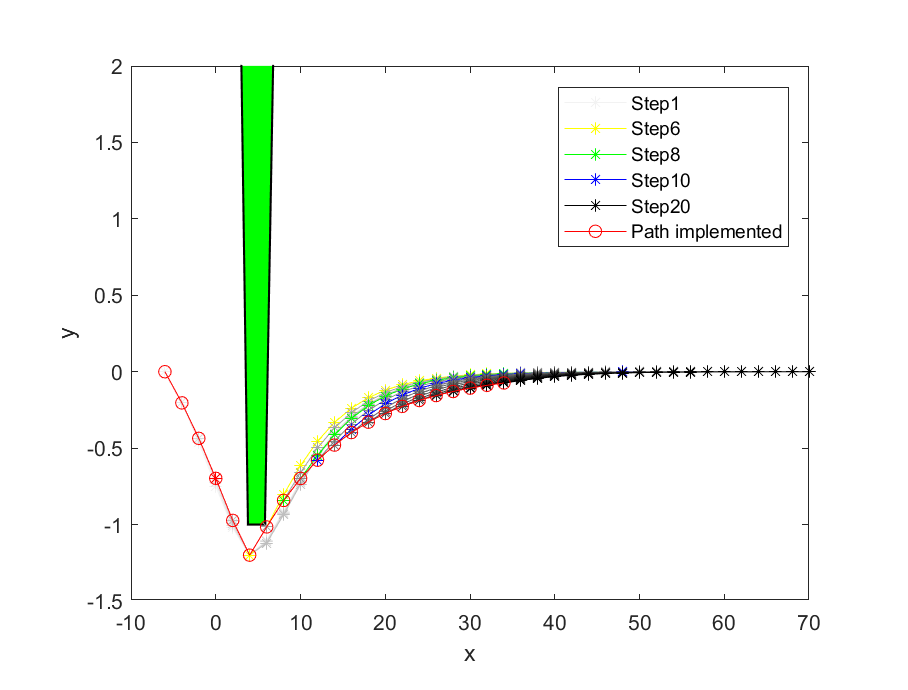
\includegraphics[width=7.5cm]{plot/1_1.eps}
\caption{Simulation result for single static obstacle.  }
\label{fig:1_1}
\end{center}
\end{figure}

%\begin{figure}[htbp]
%\begin{center}
%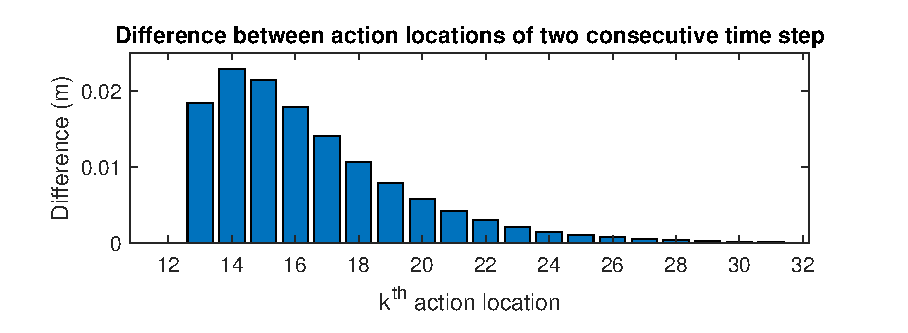
\includegraphics[width=7cm]{plot/1_2_1.eps}
%\caption{Difference between action locations of two %consecutive time step.}
%\label{fig:1_2}
%\end{center}
%\end{figure}

\begin{figure}[t]
\begin{center}
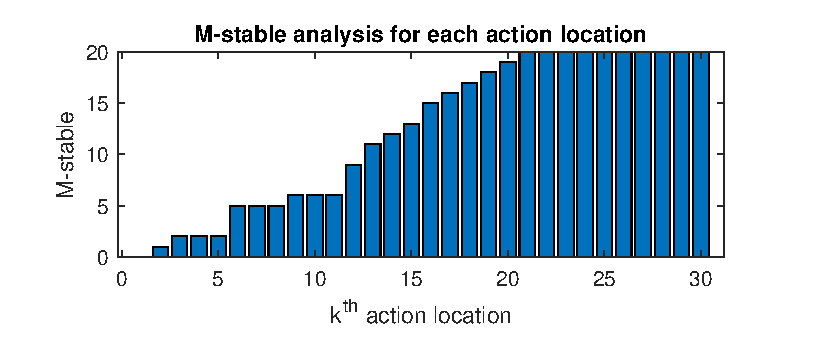
\includegraphics[width=7cm]{plot/1_2.eps}
\caption{Largest possible number $M$ for $M$-stable for each action location.}
\label{fig:1_3}
\end{center}
\end{figure}



\begin{figure}[t]
\begin{center}
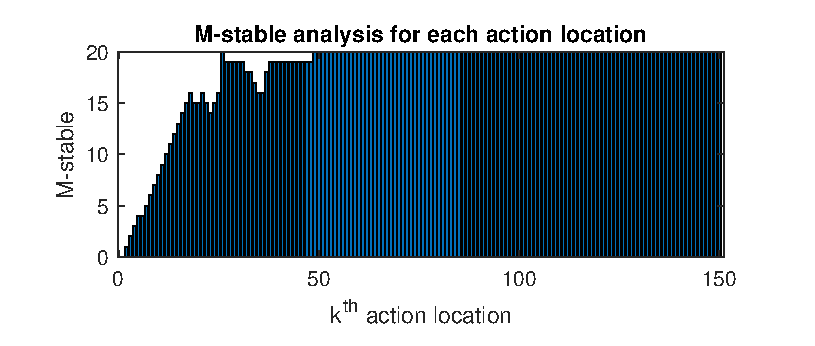
\includegraphics[width=7cm]{plot/1_4.eps}
\caption{Largest possible number $M$ for $M$-stable for each action location with increased sampling rate.}
\label{fig:1_4}
\end{center}
\end{figure}



\begin{figure}[t]
\begin{center}
\includegraphics[width=8cm]{src/1_3_path.png}
\caption{Illustration of path$_k$ (the diagonal lines).}
\label{fig:cost1}
\end{center}
\end{figure}

\begin{figure}[t]
\begin{center}
\includegraphics[width=8cm]{plot/1_3.eps}
\caption{Cost VS path.}
\label{fig:costplot}
\end{center}
\end{figure}

\subsection{Result of scenario with initially unknown static obstacle}

The result of this scenario is shown in Fig.~\ref{fig:2_1}. At the beginning, the robot does not know there exists the third obstacle on the right. After detecting the third obstacle, the robot corrects its planned trajectory to avoid the obstacle and completes its intention successfully.

The $M$-stable stability analysis discussed previously can also be applied to this scenario even though the environment is changing. Since the stability analysis strategy of this work looks close into the relation among planned action locations, i.e., every point in the trajectories, the analysis can still be done although the planned locations change a lot due to environment changes. This directly demonstrate the strength of the proposed $M$-stable analysis. The result for $M$-stable is shown in Fig.~\ref{fig:2_2}. From the plot we can see that $M$ begins to increase slower after the $16^{th}$ action location, this is exactly where the robot detects the obstacle and plans the new trajectory to avoid collision. The $26^{th}$ to the $30^{th}$ are the critical action locations, therefore, have higher $M$-stable property. After passing by the obstacle, the robot adjusts its planning to best lower the cost and then track the line with constant speed steadily. Throughout the process from detection to reaching 20-stable, the system is at least 14-stable. Once the environment stops changing, the robot system reaches to 20-stable, which agrees with the result from the static-obstacle-scenario.     


\begin{figure}[b]
\begin{center}

\subfloat[At time step t=14]{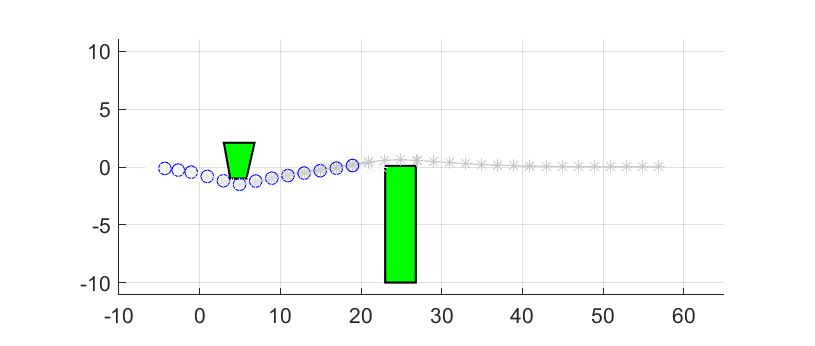
\includegraphics[width=6cm]{plot/2_1_1.eps}}
\hspace{0.5cm}
\subfloat[At time step t=15]{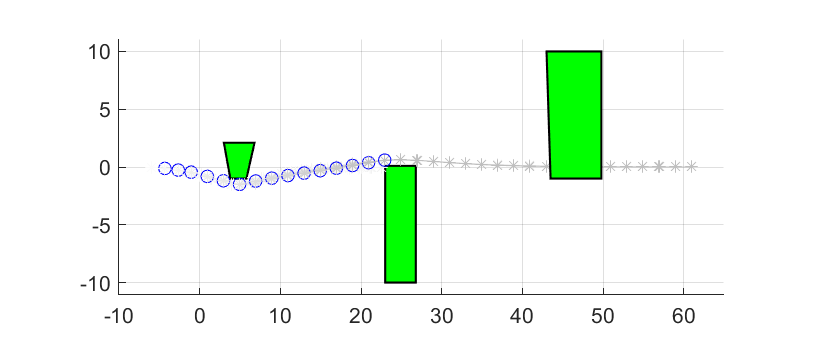
\includegraphics[width=6cm]{plot/2_1_2.eps}}
\hspace{0.5cm}
\subfloat[At time step t=19]{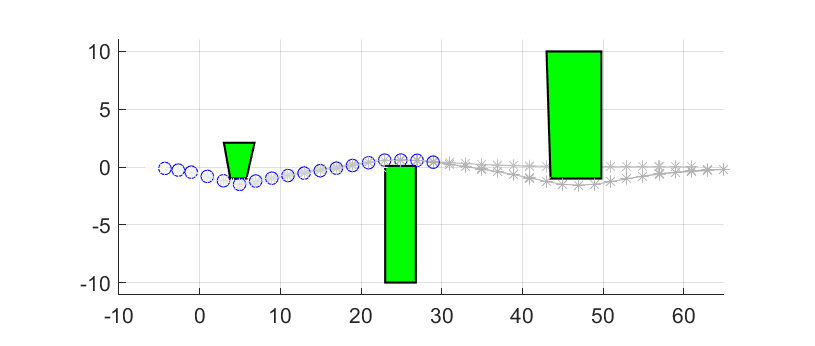
\includegraphics[width=6cm]{plot/2_1_3.eps}}
\hspace{0.5cm}
\subfloat[Final result]{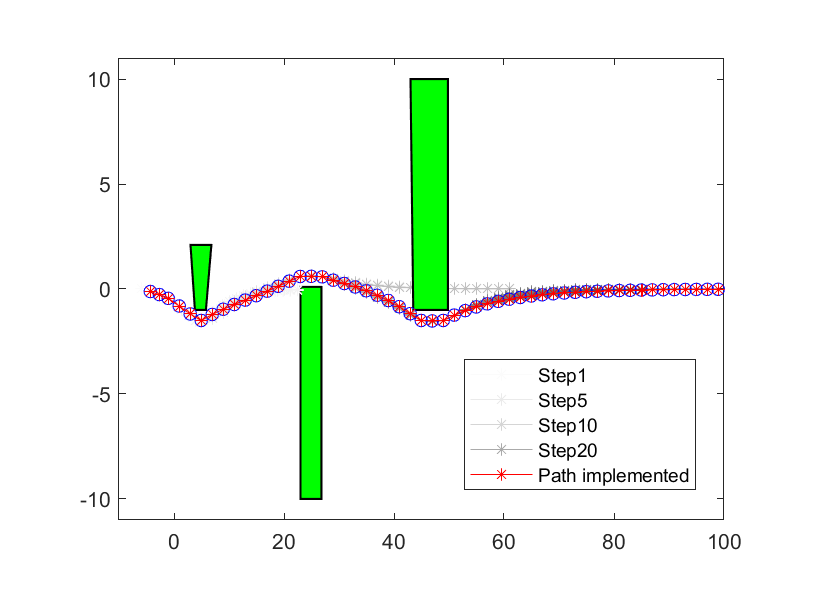
\includegraphics[width=7cm]{plot/2_1_4.eps}}
\caption{Simulation result for scenario that has initially unknown static obstacle. }
\label{fig:2_1}
\end{center}
\end{figure}

\begin{figure}[b]
\begin{center}
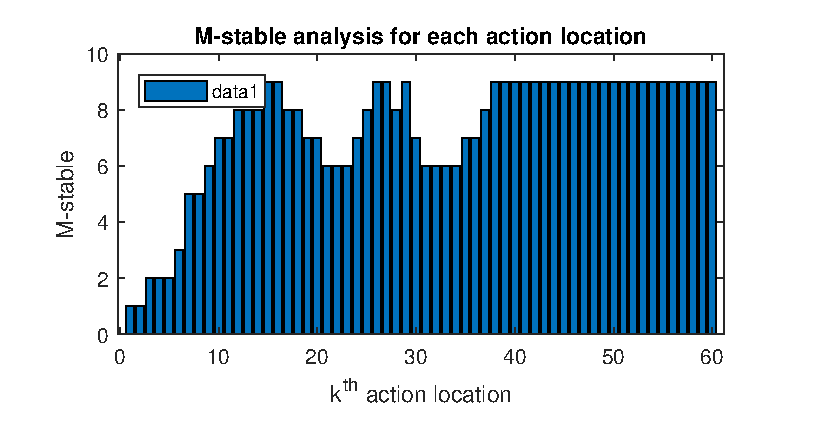
\includegraphics[width=8cm]{plot/2_2.eps}
\caption{$M$-stable analysis for scenario that has initially unknown static obstacle. }
\label{fig:2_2}
\end{center}
\end{figure}

\subsection{Result of scenario with initially unknown moving obstacle}

The result of this scenario is shown in Fig.~\ref{fig:3_1} and Fig.~\ref{fig:3_3}. In Fig.~\ref{fig:3_1}, the robot does not know there exists the third obstacle on the right at the beginning. Once the robot detects the moving obstacle, it will also assume the obstacle is moving in constant speed. Therefore, the robot is able to predict the future position of the obstacle and calculate the future action locations accordingly. Simulation result in Fig.~\ref{fig:3_1} shows that the robot avoids the obstacles successfully.

Fig.~\ref{fig:3_2} shows the $M$-stable analysis. It can be observed that there exists a similar trend as shown in Fig.~\ref{fig:2_2}. Note that in the range $k=20$ to $k=25$, $M$ decreases because of the large deviation from the trajectory planned before observing the obstacle. Also, there is a high peak in $M$ at the $26^{th}$ action location, which is the critical one at the corner of the obstacle. After passing the critical action location, the robot again has freedom to adjust its planning to best fit the cost function. And in steady environment, the robot system again reaches 9-stable. 

An even severe scenario is tested (Fig.~\ref{fig:3_3}). The obstacle will change its speed at some point after detection. In the simulation, the obstacle is originally moving along the negative $y$-axis. After time step $t=20$, the obstacle changes its speed and starts moving along the positive $y$-axis. From Fig.~\ref{fig:3_3} (b), we can see that the robot adjusts the planned trajectory to best utilize the space once it detects the speed change. The $M$-stable plot of this scenario (Fig.~\ref{fig:3_4}) is almost exactly the same as the one with no speed change. Only note that the decrease in $M$ in the range $k=20$ to $k=25$ is not as large as in the previous scenario. This is because the obstacle changes direction and the robot can avoid collision with smaller deviation form the horizontal line, thus, has more time and free space to adjust its planning to best lower the cost. The result indicates that as long as there is no sudden change accruing close before an action location is executed, the robot can best utilize the new information and successfully plan a smooth trajectory.

\subsection{Relationship between $M$ and $H$}

In industries, choosing a prediction horizon to be large enough is a common way to guarantee stability (Mayne et al., 2000). Therefore, we examined the relationship between the prediction horizon $H$ and the resulting $M$ for $M$-stability. The scenario that has unknown moving obstacle is used here. Define the largest possible $M$ at each action location as $M_{L,k}$, where $M_{L,k} = k-1$ for $k\leq H+1$, and $M_{L,k} = H$ for $k>H+1$. Fig.~\ref{fig:HMDnc} shows the difference between the largest possible $M$ that each action location can reach and the simulated $M$. The patterns of different $H$ are quite similar. In Fig.~\ref{fig:HM20nc}, however, systems with larger ($H>20$) prediction horizon reach $20$-stable (which is a guarantee that the location will not change much within 20 sampling steps before it is executed) faster than the system with $H=20$. Interestingly, all these systems reach $M=20$ in the range after $k=27$, which is the critical action location, but before $k=32$, whereas system with $H=20$ reaches $20$-stable not until after $k=45$. The same trend also happens when the unknown obstacle has speed change (Fig.~\ref{fig:HMD} and Fig.~\ref{fig:HM20}). Fig.~\ref{fig:HM} shows the smallest $M$ after $k$ reaches $H+1$ for each prediction horizon. It is clear that the smallest $M$ increase with $H$. Note that large $H$ makes the problem computationally heavy, which should be avoided if possible. We conclude that the horizon can be considered large enough if it can cover the last critical action location, in this case, when $H>27$.

\begin{figure}[t]
\begin{center}
\subfloat[At time step t=14]{\includegraphics[width=6cm]{plot/3_1_1.eps}}
\hspace{0.5cm}
\subfloat[At time step t=15]{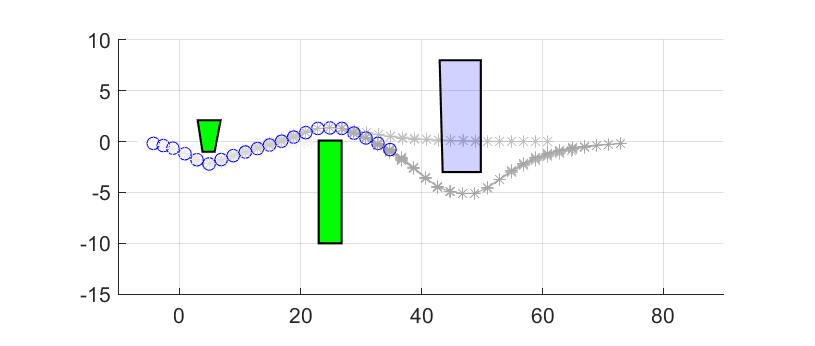
\includegraphics[width=6cm]{plot/3_1_2.eps}}
\hspace{0.5cm}
\subfloat[At time step t=27]{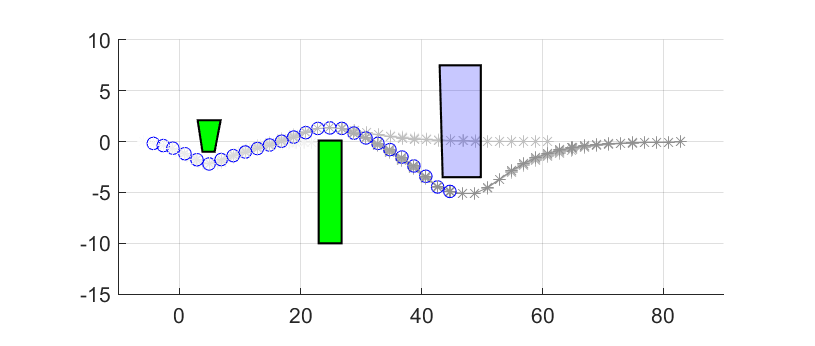
\includegraphics[width=6cm]{plot/3_1_3.eps}}
\hspace{0.5cm}
\subfloat[Final result]{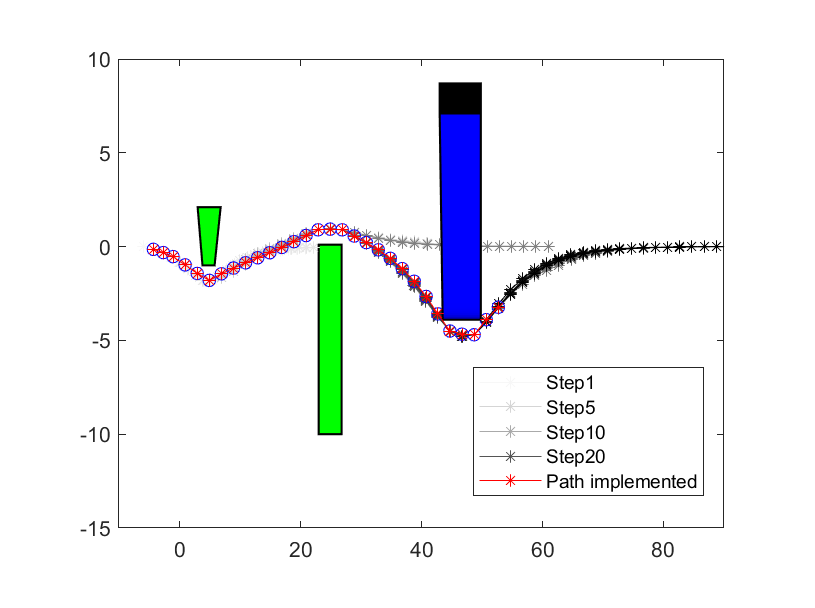
\includegraphics[width=7cm]{plot/3_1_4.eps}}
\caption{Simulation result for scenario that has initially unknown moving obstacles.}
\label{fig:3_1}
\end{center}
\end{figure}

\begin{figure}[t]
\begin{center}
\includegraphics[width=8cm]{plot/3_2.eps}
\caption{M-stable analysis for scenario that has initially unknown moving obstacles. }
\label{fig:3_2}
\end{center}
\end{figure}

\begin{figure}[t]
\begin{center}
\subfloat[At time step t=16]{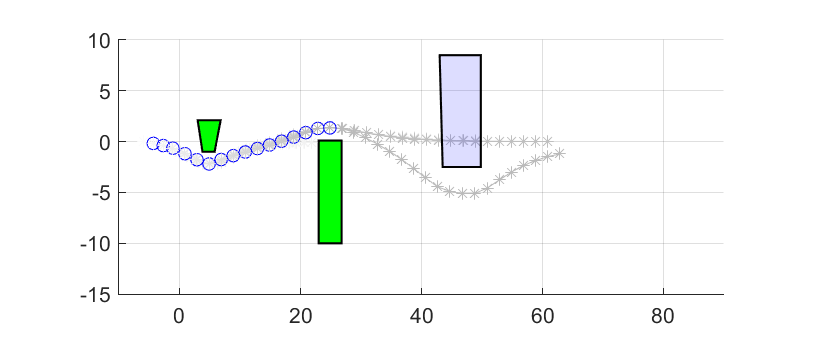
\includegraphics[width=6cm]{plot/3_3_1.eps}}
\hspace{0.5cm}
\subfloat[At time step t=21]{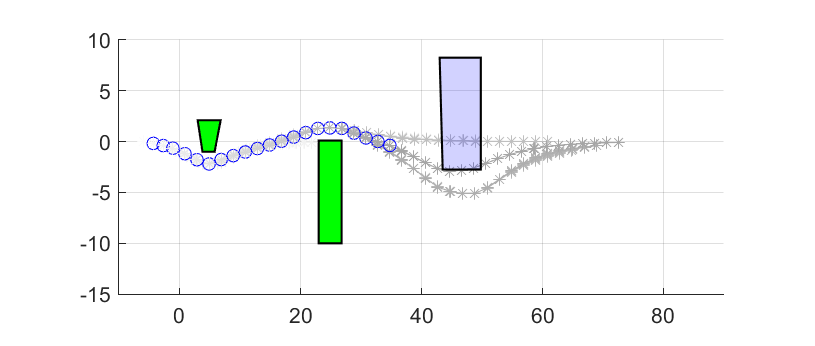
\includegraphics[width=6cm]{plot/3_3_2.eps}}
\hspace{0.5cm}
\subfloat[At time step t=27]{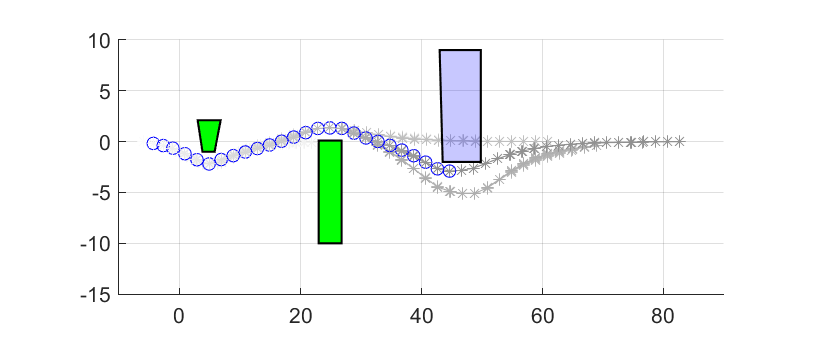
\includegraphics[width=6cm]{plot/3_3_3.eps}}
\hspace{0.5cm}
\subfloat[Final result]{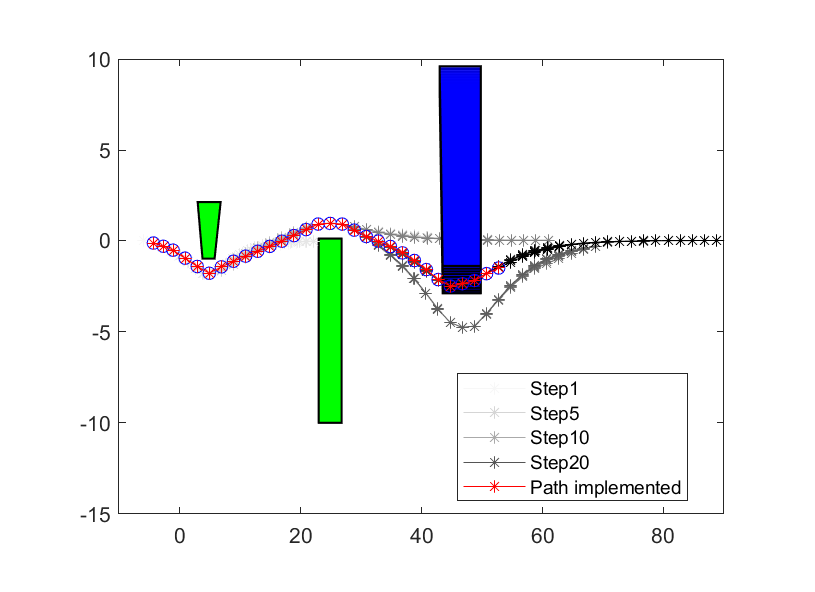
\includegraphics[width=7cm]{plot/3_3_4.eps}}
\caption{Simulation result for scenario that has initially unknown moving obstacles (with speed change).}
\label{fig:3_3}
\end{center}
\end{figure}

\begin{figure}[t]
\begin{center}
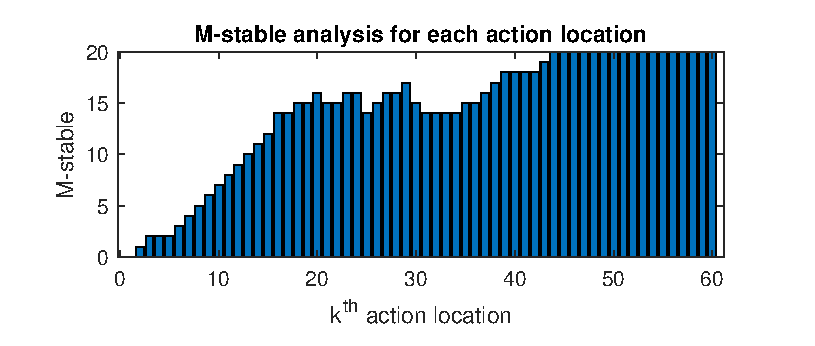
\includegraphics[width=8cm]{plot/3_4.eps}
\caption{M-stable analysis for scenario that has initially unknown moving obstacles (with speed change). }
\label{fig:3_4}
\end{center}
\end{figure}

\begin{figure}[t]
\begin{center}
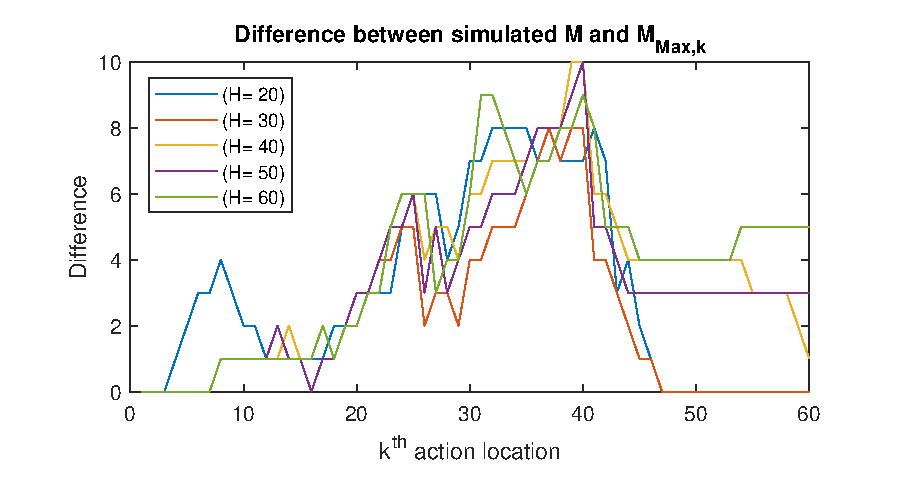
\includegraphics[width=8cm]{plot/7_nc.eps}
\caption{Difference between simulated $M$ and $M_{L,k}$. }
\label{fig:HMDnc}
\end{center}
\end{figure}

\begin{figure}[t]
\begin{center}
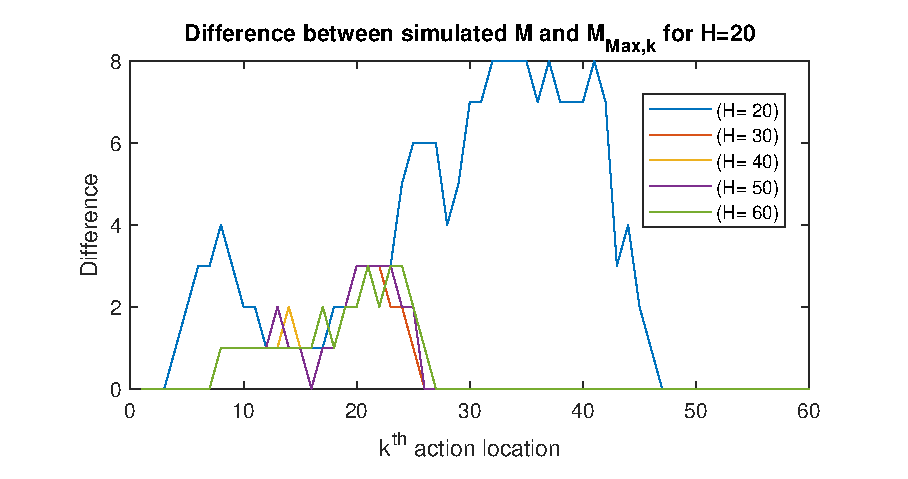
\includegraphics[width=8cm]{plot/8_nc.eps}
\caption{Difference between simulated $M$ and $M_{L,k}$ for $H=20$. }
\label{fig:HM20nc}
\end{center}
\end{figure}

\begin{figure}[t]
\begin{center}
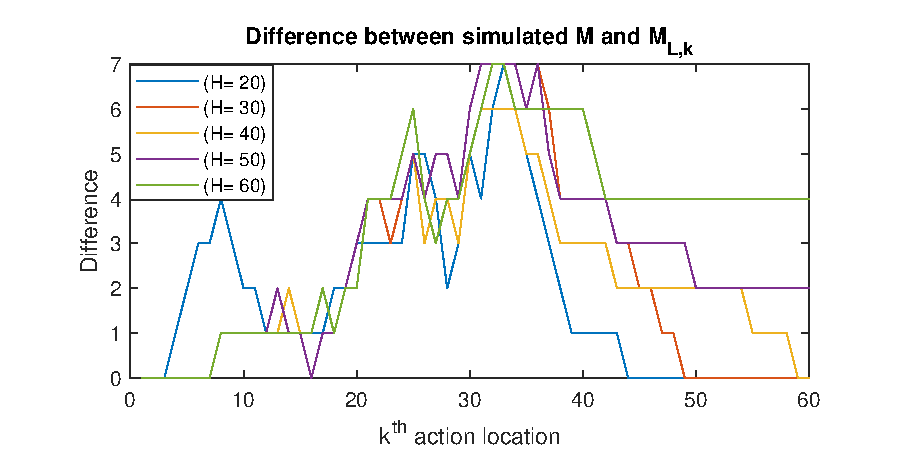
\includegraphics[width=8cm]{plot/7.eps}
\caption{Difference between simulated $M$ and $M_{L,k}$ (with speed change).}
\label{fig:HMD}
\end{center}
\end{figure}

\begin{figure}[t]
\begin{center}
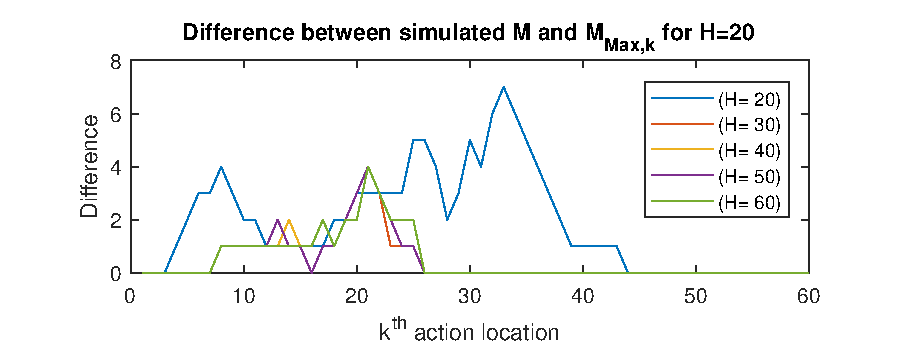
\includegraphics[width=8cm]{plot/8.eps}
\caption{Difference between simulated $M$ and $M_{L,k}$ for $H=20$ (with speed change). }
\label{fig:HM20}
\end{center}
\end{figure}


\begin{figure}[t]
\begin{center}
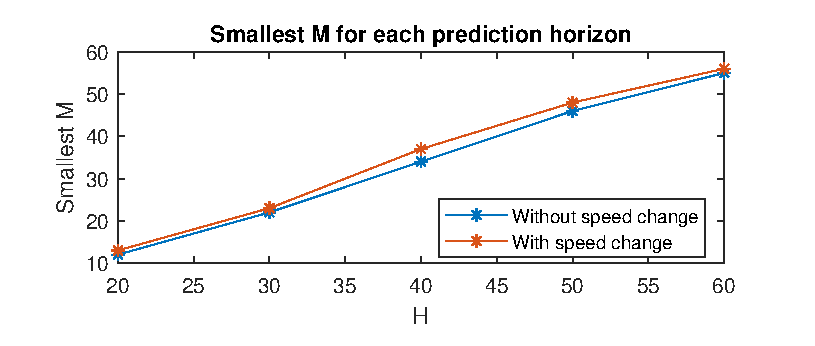
\includegraphics[width=8cm]{plot/9.eps}
\caption{Smallest $M$ for each prediction horizon. }
\label{fig:HM}
\end{center}
\end{figure}



\section{Conclusion}

This paper proposed a new method of analyzing stability properties for non-convex MPC. The proposed method, $M$-stablility analysis, considered the difference of each action location planned at consecutive time steps. We said the action location $k$ is $m$-stable  if there is smaller and smaller change between consecutive time steps after time step $k-m$. Simulation  results showed that a robot that implemented the CFS algorithm in the MPC framework was capable of dealing with dynamic environment as long as the changes in the environment was predictable. The stability analysis using $M$-stable (and also other methods for static case) was performed. It was shown that the robot had decent stability properties. In the future, we will include the robot dynamics in to the problem formulation and complete the theoretical proof for $M$-stable analysis.



%\begin{ack}
%Place acknowledgments here.
%\end{ack}


 
% in the appendices.
\begin{thebibliography}{xx}  % you can also add the bibliography by hand

\bibitem[Able(1956)]{Abl:56}
N. Wu and M.C. Zhou.
\newblock Modeling and deadlock control of automated guided vehicle systems.
\newblock \emph{ IEEE/ASME Transactions on Mechatronics }, Volume: 9, Issue: 1:\penalty0 50 - 57, 2004.

\bibitem[Able(1956)]{Abl:56}
J. Wang, J. Steiber, and B. Surampudi.
\newblock Autonomous ground vehicle control system for high-speed and safe operation.
\newblock \emph{ American Control Conference }, 2008.


\bibitem[Able(1956)]{Abl:56}
F. Oleari, M. Magnani, and D. Ronzoni.
\newblock Industrial AGVs: Toward a pervasive diffusion in modern factory warehouses.
\newblock \emph{ IEEE/ICCP }, 2014.


\bibitem[Able(1956)]{Abl:56}
J.B. Rawlings.
\newblock Tutorial: model predictive control technology.
\newblock \emph{  American Control Conference }, 1999.

\bibitem[Able(1956)]{Abl:56}
D.Q. Mayne, J.B. Rawlingsb, C.V. Raob, and P.O.M. Scokaertc.
\newblock Constrained model predictive control: Stability and optimality.
\newblock \emph{  Automatica }, Volume: 36, Issue: 6:\penalty0 789 - 814, 2000.

\bibitem[Able(1956)]{Abl:56}
D. Limon, T. Alamo, and F. Salas.
\newblock On the stability of constrained MPC without terminal constraint.
\newblock \emph{   IEEE Transactions on Automatic Control }, Volume: 51, Issue: 5:\penalty0 832 - 836, 2006.

\bibitem[Able(1956)]{Abl:56}
S.S. Dughman and J.A. Rossiter.
\newblock A survey of guaranteeing feasibility and stability in MPC during target changes.
\newblock \emph{   IFAC-PapersOnLine }, Volume: 48, Issue: 8:\penalty0 813 - 818, 2015.

\bibitem[Able(1956)]{Abl:56}
L. Zhanga, S. Zhuanga, and R.D. Braatzb.
\newblock Switched model predictive control of switched linear systems:
Feasibility, stability and robustness.
\newblock \emph{  Automatica  }, Volume: 67\penalty0 8 - 21, 2016.

\bibitem[Able(1956)]{Abl:56}
A. Bocciaa, L. Grüneb, and K. Worthmannc.
\newblock Stability and feasibility of state constrained MPC without stabilizing terminal constraints.
\newblock \emph{  Systems and Control Letters  }, Volume: 72\penalty0 14 - 21, 2014.



\bibitem[Able(1956)]{Abl:56}
F. Borrelli.
\newblock Stabilization of 2-D Spider Crane with Non-Convex State Constraints using MPC.
\newblock \emph{ Inderscience Enterprises Limited  }, Volume: 3, Issue: 2\penalty0 265 - 290, 2006.

\bibitem[Able(1956)]{Abl:56}
T.G. Hovgaard, L.F.S. Larsen, J.B. Jørgensen, and S. Boyd.
\newblock Nonconvex Model Predictive Control for Commercial Refrigeration.
\newblock \emph{ IFAC Proceedings Volumes  }, Volume: 45, Issue: 17\penalty0 514 - 521, 2012.

\bibitem[Able(1956)]{Abl:56}
C. Liu, C.Y. Lin, and M. Tomizuka.
\newblock The Convex Feasible Set Algorithm for Real Time Optimization in Motion Planning.
\newblock under review in \emph{ SIAM Journal on Control and Optimization}, arXiv:1709.00627, 2016.




%\bibitem[Able et~al.(1954)Able, Tagg, and Rush]{AbTaRu:54}
%B.C. Able, R.A. Tagg, and M.~Rush.
%\newblock Enzyme-catalyzed cellular transanimations.
%\newblock In A.F. Round, editor, \emph{Advances in Enzymology}, volume~2, pages
%  125--247. Academic Press, New York, 3rd edition, 1954.

%\bibitem[Keohane(1958)]{Keo:58}
%R.~Keohane.
%\newblock \emph{Power and Interdependence: World Politics in Transitions}.
%\newblock Little, Brown \& Co., Boston, 1958.

%\bibitem[Powers(1985)]{Pow:85}
%T.~Powers.
%\newblock Is there a way out?
%\newblock \emph{Harpers}, pages 35--47, June 1985.

%\bibitem[Soukhanov(1992)]{Heritage:92}
%A.~H. Soukhanov, editor.
%\newblock \emph{{The American Heritage. Dictionary of the American Language}}.
%\newblock Houghton Mifflin Company, 1992.

\end{thebibliography}
\end{document}
